\documentclass[11pt]{article}
\usepackage[a4paper, left=1in, right=1in, top=1in, bottom=1in]{geometry}
\newcommand*{\authorfont}{\fontfamily{phv}\selectfont}
\usepackage[english, greek, main=english]{babel}
\usepackage[]{mathptmx}
\usepackage[LGR,T1]{fontenc}
\usepackage[utf8]{inputenc}
\usepackage[page,toc,titletoc,title]{appendix}  % appendix, table of contents
\usepackage{enumitem}  % package for adjusting itemize sep
\usepackage{amssymb}  % extra math fonts, like \mathbb, \mathcal
\usepackage{amsmath}
\usepackage{amsthm}
\theoremstyle{definition}
\newtheorem{definition}{Definition}
\newtheorem{example}[definition]{Example}  % example numbering depends on definition
\usepackage{abstract}
\renewcommand{\abstractname}{}    % clear the title
\renewcommand{\absnamepos}{empty} % originally center
\usepackage{tikz}
\usepackage{pgfplots}
\usepackage{xcolor}
\pgfplotsset{compat=1.16}
\usepackage{tcolorbox}
\usepackage{listings}
\usepackage{subcaption}
\usepackage{booktabs}
\usepackage{varwidth}
\usepackage[export]{adjustbox}
\usetikzlibrary{arrows}

\renewenvironment{abstract}
 {{%
    \setlength{\leftmargin}{0mm}
    \setlength{\rightmargin}{\leftmargin}%
  }%
  \relax}
 {\endlist}

\makeatletter
\def\@maketitle{%
  \newpage
%  \null
%  \vskip 2em%
%  \begin{center}%
  \let \footnote \thanks
    {\fontsize{18}{20}\selectfont\raggedright  \setlength{\parindent}{0pt} \@title \par}%
}
%\fi
\makeatother




\setcounter{secnumdepth}{0}

\usepackage{color}
\usepackage{fancyvrb}
\newcommand{\VerbBar}{|}
\newcommand{\VERB}{\Verb[commandchars=\\\{\}]}
\DefineVerbatimEnvironment{Highlighting}{Verbatim}{commandchars=\\\{\}}
% Add ',fontsize=\small' for more characters per line
\usepackage{framed}
\definecolor{shadecolor}{RGB}{248,248,248}
\newenvironment{Shaded}{\begin{snugshade}}{\end{snugshade}}
\newcommand{\AlertTok}[1]{\textcolor[rgb]{0.94,0.16,0.16}{#1}}
\newcommand{\AnnotationTok}[1]{\textcolor[rgb]{0.56,0.35,0.01}{\textbf{\textit{#1}}}}
\newcommand{\AttributeTok}[1]{\textcolor[rgb]{0.77,0.63,0.00}{#1}}
\newcommand{\BaseNTok}[1]{\textcolor[rgb]{0.00,0.00,0.81}{#1}}
\newcommand{\BuiltInTok}[1]{#1}
\newcommand{\CharTok}[1]{\textcolor[rgb]{0.31,0.60,0.02}{#1}}
\newcommand{\CommentTok}[1]{\textcolor[rgb]{0.56,0.35,0.01}{\textit{#1}}}
\newcommand{\CommentVarTok}[1]{\textcolor[rgb]{0.56,0.35,0.01}{\textbf{\textit{#1}}}}
\newcommand{\ConstantTok}[1]{\textcolor[rgb]{0.00,0.00,0.00}{#1}}
\newcommand{\ControlFlowTok}[1]{\textcolor[rgb]{0.13,0.29,0.53}{\textbf{#1}}}
\newcommand{\DataTypeTok}[1]{\textcolor[rgb]{0.13,0.29,0.53}{#1}}
\newcommand{\DecValTok}[1]{\textcolor[rgb]{0.00,0.00,0.81}{#1}}
\newcommand{\DocumentationTok}[1]{\textcolor[rgb]{0.56,0.35,0.01}{\textbf{\textit{#1}}}}
\newcommand{\ErrorTok}[1]{\textcolor[rgb]{0.64,0.00,0.00}{\textbf{#1}}}
\newcommand{\ExtensionTok}[1]{#1}
\newcommand{\FloatTok}[1]{\textcolor[rgb]{0.00,0.00,0.81}{#1}}
\newcommand{\FunctionTok}[1]{\textcolor[rgb]{0.00,0.00,0.00}{#1}}
\newcommand{\ImportTok}[1]{#1}
\newcommand{\InformationTok}[1]{\textcolor[rgb]{0.56,0.35,0.01}{\textbf{\textit{#1}}}}
\newcommand{\KeywordTok}[1]{\textcolor[rgb]{0.13,0.29,0.53}{\textbf{#1}}}
\newcommand{\NormalTok}[1]{#1}
\newcommand{\OperatorTok}[1]{\textcolor[rgb]{0.81,0.36,0.00}{\textbf{#1}}}
\newcommand{\OtherTok}[1]{\textcolor[rgb]{0.56,0.35,0.01}{#1}}
\newcommand{\PreprocessorTok}[1]{\textcolor[rgb]{0.56,0.35,0.01}{\textit{#1}}}
\newcommand{\RegionMarkerTok}[1]{#1}
\newcommand{\SpecialCharTok}[1]{\textcolor[rgb]{0.00,0.00,0.00}{#1}}
\newcommand{\SpecialStringTok}[1]{\textcolor[rgb]{0.31,0.60,0.02}{#1}}
\newcommand{\StringTok}[1]{\textcolor[rgb]{0.31,0.60,0.02}{#1}}
\newcommand{\VariableTok}[1]{\textcolor[rgb]{0.00,0.00,0.00}{#1}}
\newcommand{\VerbatimStringTok}[1]{\textcolor[rgb]{0.31,0.60,0.02}{#1}}
\newcommand{\WarningTok}[1]{\textcolor[rgb]{0.56,0.35,0.01}{\textbf{\textit{#1}}}}

\usepackage{graphicx,grffile}
\makeatletter
\def\maxwidth{\ifdim\Gin@nat@width>\linewidth\linewidth\else\Gin@nat@width\fi}
\def\maxheight{\ifdim\Gin@nat@height>\textheight\textheight\else\Gin@nat@height\fi}
\makeatother
% Scale images if necessary, so that they will not overflow the page
% margins by default, and it is still possible to overwrite the defaults
% using explicit options in \includegraphics[width, height, ...]{}
\setkeys{Gin}{width=\maxwidth,height=\maxheight,keepaspectratio}

\usepackage{titlesec}

\titleformat*{\section}{\normalsize\bfseries}
\titleformat*{\subsection}{\normalsize\itshape}
\titleformat*{\subsubsection}{\normalsize\itshape}
\titleformat*{\paragraph}{\normalsize\itshape}
\titleformat*{\subparagraph}{\normalsize\itshape}

\usepackage{natbib}
\usepackage[strings]{underscore} % protect underscores in most circumstances

\newtheorem{hypothesis}{Hypothesis}
\usepackage{setspace}

% set default figure placement to htbp
\makeatletter
\def\fps@figure{htbp}
\makeatother

\usepackage{hyperref}

% move the hyperref stuff down here, after header-includes, to allow for - \usepackage{hyperref}

\makeatletter
\@ifpackageloaded{hyperref}{}{%
\ifxetex
  \PassOptionsToPackage{hyphens}{url}\usepackage[setpagesize=false, % page size defined by xetex
              unicode=false, % unicode breaks when used with xetex
              xetex]{hyperref}
\else
  \PassOptionsToPackage{hyphens}{url}\usepackage[draft,unicode=true]{hyperref}
\fi
}

\@ifpackageloaded{color}{
    \PassOptionsToPackage{usenames,dvipsnames}{color}
}{%
    \usepackage[usenames,dvipsnames]{color}
}
\makeatother
\hypersetup{breaklinks=true,
            bookmarks=true,
            pdfauthor={Steven V. Miller (Clemson University)},
             pdfkeywords = {pandoc, r markdown, knitr},  
            pdftitle={A Pandoc Markdown Article Starter and Template},
            colorlinks=true,
            citecolor=blue,
            urlcolor=blue,
            linkcolor=magenta,
            pdfborder={0 0 0}}
\urlstyle{same}  % don't use monospace font for urls

% Add an option for endnotes. -----


% add tightlist ----------
\providecommand{\tightlist}{%
\setlength{\itemsep}{0pt}\setlength{\parskip}{0pt}}

% add some other packages ----------

% \usepackage{multicol}
% This should regulate where figures float
% See: https://tex.stackexchange.com/questions/2275/keeping-tables-figures-close-to-where-they-are-mentioned
\usepackage[section]{placeins}


% Title and author

\title{Hands-On Data Analysis for ININ Using R}

\author{\Large Prof. Dr. Cornelia Storz, M.Sc. Fei (Michael) Wang\vspace{0.05in} \newline\normalsize\emph{Management and Microeconomics, Goethe-Universität Frankfurt}  }

\date{}

% colback=white,
% colframe=white!50!black, 
% title = {Sample space: countable or uncountable?}, 
% fonttitle = \large

% set tcolorbox environment
\newtcolorbox{mybox}[1]
{
  colframe = white!50!black,
  colback  = white,
  fonttitle = \large, 
  title    = {#1}
}

\xdefinecolor{gray}{rgb}{0.4,0.4,0.4}
\xdefinecolor{blue}{RGB}{58,95,205}% R's royalblue3; #3A5FCD

\lstset{% setup listings
	language=R,% set programming language
	basicstyle=\ttfamily\small,% basic font style
	keywordstyle=\color{blue},% keyword style
        commentstyle=\color{gray},% comment style
	numbers=left,% display line numbers on the left side
	numberstyle=\scriptsize,% use small line numbers
	numbersep=10pt,% space between line numbers and code
	tabsize=3,% sizes of tabs
  commentstyle=\itshape\color{green!50!gray},
  frame=single,% single frame around code
	showstringspaces=false,% do not replace spaces in strings by a certain character
	captionpos=b,% positioning of the caption below
        breaklines=true,% automatic line breaking
        escapeinside={(*}{*)},% escaping to LaTeX
        fancyvrb=true,% verbatim code is typset by listings
        extendedchars=false,% prohibit extended chars (chars of codes 128--255)
        literate={"}{{\texttt{"}}}1{<-}{{$\bm\leftarrow$}}1{<<-}{{$\bm\twoheadleftarrow$}}1
        {~}{{$\bm\sim$}}1{<=}{{$\bm\le$}}1{>=}{{$\bm\ge$}}1{!=}{{$\bm\neq$}}1{^}{{$^{\bm\wedge}$}}1,% item to replace, text, length of chars
        alsoletter={.<-},% becomes a letter
        alsoother={$},% becomes other
        otherkeywords={!=, ~, $, \&, \%/\%, \%*\%, \%\%, <-, <<-, /},% other keywords
        deletekeywords={c}% remove keywords
}



%----------------------------begin document--------------------------------%

\begin{document}
	
% \pagenumbering{arabic}% resets `page` counter to 1 
%
% \maketitle

{% \usefont{T1}{pnc}{m}{n}
\setlength{\parindent}{0pt}
\thispagestyle{plain}
{\fontsize{18}{20}\selectfont\raggedright 
\maketitle  % title \par  

}

{
   \vskip 13.5pt\relax \normalsize\fontsize{11}{12} 
   \authorfont Prof. Dr. Cornelia Storz, M.Sc. Fei (Michael) Wang \\
   \\ 
    \emph{\small Management and Microeconomics, Goethe-Universität Frankfurt}   
}

}



\begin{abstract}
    \hbox{\vrule height .2pt width 39.14pc}
    \vskip 8.5pt % \small 

\noindent This document was prepared for students who are taking ININ course and
planning to take the exam. It is a collection of notes and codes for the
course. The notes are based on the tutorials we had in the course. I am trying
to make it concise and easy to understand. I hope it can help you to review
the course and prepare for the exam. \textit{We are living in a very noisy world,
therefore let's keep it simple and clear.} I setup a challenge for myself to
deliver a clear and concise review notes within 15 pages. This brings the trade-off,
which means some figures and tables are not included in the notes. Therefore,
you have to run the codes to see the results.  

\vskip 6pt 

\noindent I hope you enjoy reading it. I also hope you will have this notes with you
whenever you want to do some data analysis. If one day, you still refer to this
notes and find it still useful, I would be very happy to hear that.

 

\vskip 8.5pt \noindent \emph{Keywords}: econometrics, data analysis, regression models, 
empirical research, innovation, management  \par
\hbox{\vrule height .2pt width 39.14pc}

\end{abstract}

\vskip -8.5pt

 % removetitleabstract

\noindent  

% table of contents
\pagenumbering{roman}
\hypersetup{linkcolor=black}
\setcounter{tocdepth}{3}
\tableofcontents


\newpage
\pagenumbering{arabic}
\setcounter{page}{1}
\section{1 Introduction}

All statistical or econometric or machine learning models are based on 
the following assumptions:

\begin{itemize}
\tightlist
\item there are something we know - \textbf{data}
\item and something we don't know - \textbf{error} \(\epsilon\).
\end{itemize}

In summary, according to confucius, \textit{to know what we know and what we do not know}, 
that is called \textbf{wisdom}. Or like Plato said, \textit{I know that I know nothing}.
To help you to review the course, the notes will be organized as follows:

\begin{enumerate}
\tightlist 
  \item \textbf{Data}: using \texttt{data.table} to get familiar with the data
  \item \textbf{Simple linear regression}: how to estimate a simple linear regression model, how to interpret the results
  \item \textbf{Multiple linear regression}: how to estimate a multiple linear regression model, how to interpret the results, how to test the model
  \item \textbf{Introduction to logistic regression}: why do we need logistic regression
  \item \textbf{Data manipulation}: will not be tested in the exam, but it is very useful for your future work or research
\end{enumerate}



\section{2 Introduction to Data and \texttt{data.table}}



Broadly speaking, there are two kinds of data: \textbf{structured data} and 
\textbf{unstructured data}. 
Structured data is data that has a structure, such as a table, 
whereas unstructured data is data that does not have a structure, 
such as a text file. In this course, we focus on structured data. 
This means all the data we will use look like tables, such as the following one:


\begin{figure}
  \centering
  \includegraphics[width=0.97\textwidth]{../drawio/R-data-table-illustration.png}
\end{figure}


The basic syntax of data.table is summarized in the following illustration. 
\textbf{You will not be tested on the syntax of data.table in the exam}. However, 
you will be tested on the underlying concepts of data.table, such as the
type of variables (integer, character, factor, etc.). In the future if
you will be working as a data scientist, you can use data.table to do 
big data analysis. You will need to know the syntax of data.table for 
practical use not for the exam.


\begin{figure}
    \centering
    \includegraphics[width=0.97\textwidth]{../drawio/R-data-table-illustration2.png}
\end{figure}

Let's start from installing and loarding the packages we need for the course.

\lstset{language=R}   

\begin{lstlisting}
# install packages
install.packages("stargazer")
# install ISLR if you don't have it
# install.packages("ISLR")
install.packages("corrplot")
# sometimes you need to install other packages
# hopefully you can figure it out by yourself
\end{lstlisting}

After you install the packages, you can load them into R.

\begin{lstlisting}
# library for data analysis
library(data.table)
library(magrittr)
library(ggplot2)
library(knitr)
library(stargazer)
library(MASS)
library(ISLR)
library(corrplot)
\end{lstlisting}

Now, we can load the data into R and manipulate the data.

\begin{lstlisting}
# read the dataset
cis <- fread("https://shorturl.at/wBESZ")
# check structure of the dataset
str(cis)
# check the first 10 rows of the dataset
head(cis, 10)
# check the number of missing values in each column
cis %>%
    .[, .SD, .SDcols = is.double] %>%
    # check the number of missing values in each column
    sapply(function(x) sum(is.na(x))) %>%
    # sort the number of missing values in each column
    sort(decreasing = TRUE) %>%
    # convert to data.table and keep rownames as a column
    as.data.table(keep.rownames = TRUE) %>%
    # set variable names
    setnames(c("variables", "Numbe of NAs")) %>%
    # check the first 10 
    head(10) %>%
    kable("pipe)
\end{lstlisting}


\subsection{2.1 Data Visualization}

It is important to visualize the data before you start to do the analysis.
To choose the right figure, you need to know the type of variables. Here is
the summary:

\begin{itemize}
\tightlist
\item \textbf{Categorical variables}: bar chart, pie chart, etc.
\item \textbf{Continuous variables}: histogram, boxplot, etc.
\item \textbf{Categorical vs. continuous variables}: boxplot or violin or histogram with different colors
\end{itemize}

Here is a demo of how to visualize the data. You can try to run the code
and see the results.

\begin{lstlisting}
# four figures in one page
# bar chart, histogram, box plot and box plot compared
# figure size
options(repr.plot.width = 10, repr.plot.height = 10)
par(mfrow = c(2, 2))
cis %>%
    # group by branche and .N calculates the number of frequency
    .[, .N, by = branche] %>%
    # order it in a descending way
    .[order(-N)] %>%
    # get the top 10 branche (industry)
    head(10) %>%
    # plot it
    with(pie(N, labels = branche, main = "Distribution of Industries"))

# histgorma for number of employees
cis %>%
    with(hist(bges, main = "number of employees"))
# boxplot for sales
cis %>%
    with(boxplot(um18,  main = "Boxplot of Sales in 2018"))
# boxplot for log(1+sales)
cis %>%
    with(boxplot(log(1+um18), main = "Boxplot of Log Transform "))
\end{lstlisting}

When you visualize the data, it is important to check two things for 
continuous variables:
\begin{itemize}
\tightlist
\item \textbf{shape}: whether the distribution is symmetric or skewed (ideally, we prefer symmetric distribution)
\item \textbf{outliers}: outliers are extreme values that deviate from other observations on data , they may indicate a variability in a measurement, experimental errors or a novelty.
\end{itemize}

\subsection{2.2 Log Transformation}

Log transformation is a very useful tool to deal with skewed data.
When you have a skewed data, you can try to log transform it. However, it
could be tricky. You need to know the underlying theory of log transformation.
Generally speaking, log transformation is used to make the data more symmetric.
To avoid the negative values, we usually use \(\log(1+x)\) instead of \(\log(x)\).

\begin{lstlisting}
# log transform
options(repr.plot.width = 10, repr.plot.height = 10)
par(mfrow = c(2, 2))
cis %>%
    with(hist(um18, main = "Histgoram of Sales (2018)"))

cis %>%
    with(hist(log(1+um18), main = "Histogram of Log (1+sales)"))

cis %>%
    with(boxplot(um18, main = "Boxplot of Sales (2018)"))
cis %>%
    with(boxplot(log(1+um18), main = "Boxplot of Log Transform "))
\end{lstlisting}


\begin{figure}
  \centering
  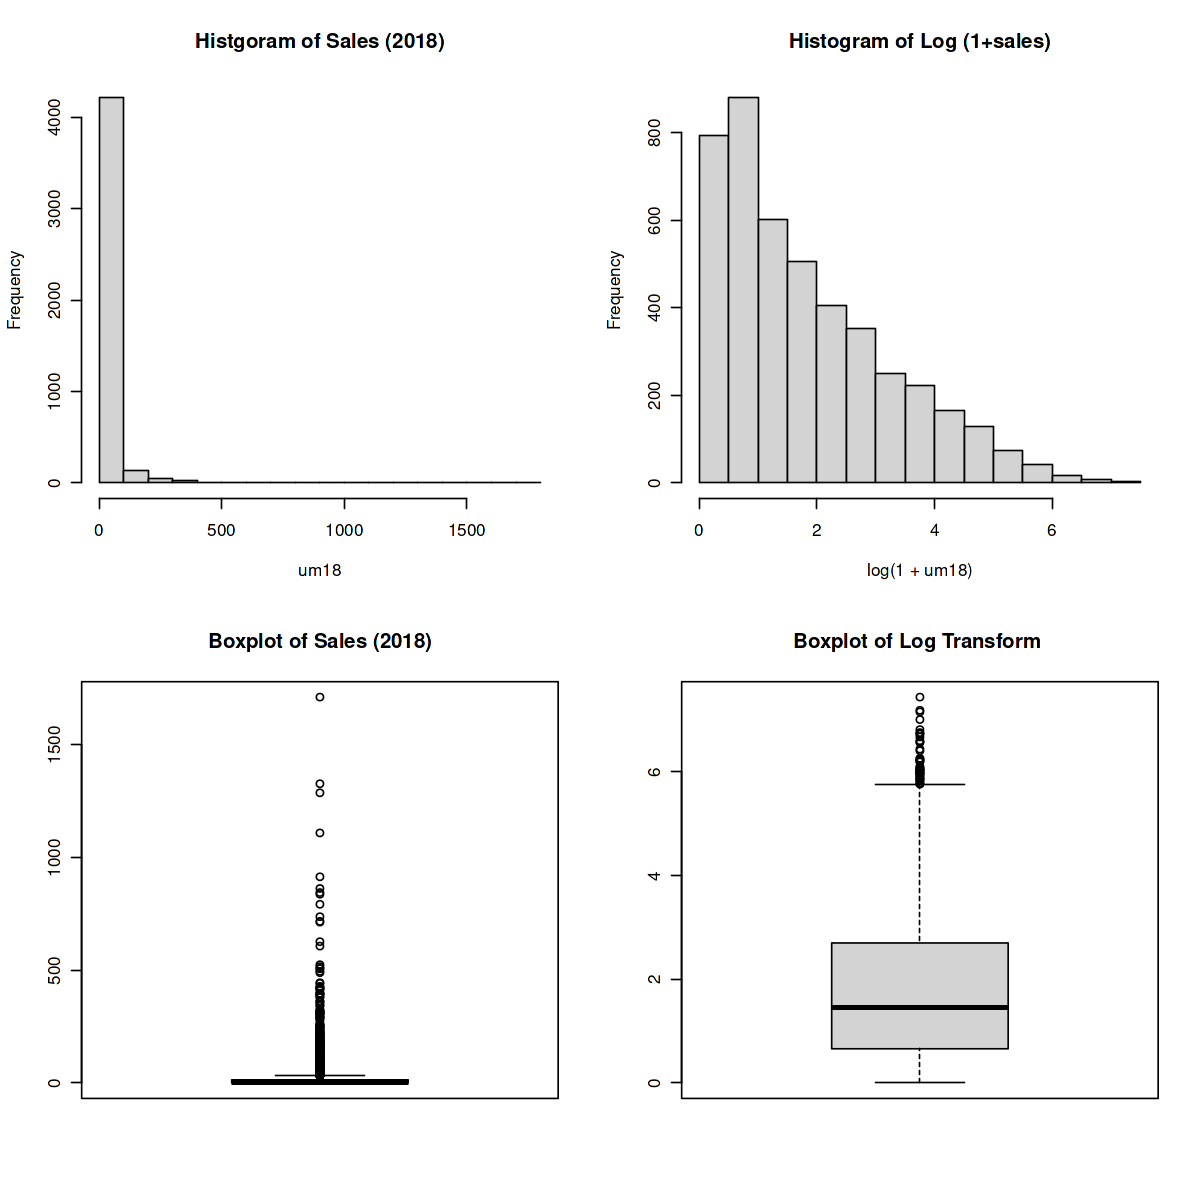
\includegraphics[width=0.9\textwidth]{./figures/vis_figure2.png}
  \caption{Log transformation of sales}
\end{figure}

When we fit a linear regression model, if dependent variable is continuous, 
we prefer the dependent variable to be normally distributed. 
So, we need to check whether the dependent variable is normally distributed. 
If not, we could use some transformation to make it normally distributed. 
As we have covered in the tutorials, there are two main distributions you need to know:

\begin{itemize}
  \tightlist 
  \item normal distribution (Gaussian distribution)
  \item binomial distribution
\end{itemize}

Possion distribution will not be tested in the exam.

\begin{figure}
  \centering
  \includegraphics[width=0.99\textwidth]{../images/binomial-to-poisson2.png}
\end{figure}


\section{3 Simple Linear Regression}

In our tutorials, we follow the following analytic frapmework:


\begin{table}[!h]
  \centering
  \begin{tabular}{lcl}
    \toprule 
  \multicolumn{1}{l}{} & Number of Variables & \multicolumn{1}{c}{Focus}                     \\
  \hline 
  Univariate           & 1                   & Distribution: Gaussian or Other distributions \\
  Bivariate            & 2                   & Correlation or contingency table                          \\
  Multivariate         & 3 or more           & Regression or classification                          \\ 
  \hline                                          
  \end{tabular}
\end{table}

Allow me to quote again:

\begin{quote}
  \textit{Dao begets One (such as emptyness, or existence, or the individual),
  One begets Two (yin and yang, or the binary), Two begets Three (the trinity, or heaven, earth and Huamn
  beings), and Three begets all things(the world).} -- Dao De Jing of Lao Tzu
\end{quote}

Many exam questions will be related to regression analysis. 
So, please pay attention to this section and the next one too. Before we run a regression analysis, 
let's first understand the basic concepts of regression analysis via simulation.

We know that the relationship between \texttt{weight} and \texttt{height} is 
roughly linear and positive. We will use this relationship to simulate the 
data. When we simulate the data, we will add some
random nosie to the data as there is no perfect linear relationship
between\texttt{weight} and \texttt{height}.
To make you understand the concept, I will simulate the data step by step: 

\begin{itemize}
\tightlist
\item scenario 1: no noise (perfect linear relationship)
\item scenario 2: add some noise (not perfect linear relationship)
\item scenario 3: add some outliers (not perfect linear relationship)
\end{itemize}

Please run the following code and check the results. You could only learn 
those concepts by doing it yourself.

\begin{lstlisting}
# simulate weight and height
# generate 900 random numbers from normal distribution
# mean =  175cm and sd = 10cm
height <- rnorm(900, mean = 175, sd = 10)
# plot histogram
hist(height, breaks = 20, xlab="Height (cm)",
             main="Histogram of Height")
\end{lstlisting}


Now, we have the height, we assume that there is a linear relationship between 
height and weight, which has the following form:

$$
weight = \beta_0 + \beta_1 \times height
$$

Here we set $\beta_0 = 55$ and $\beta_1 = 0.1$. This means that if the height increases by 1 cm, the weight will increase by 0.1 kg.

$$
weight = 55 + 0.1 \times height
$$

It has the format:

$$
y = b + ax
$$

\begin{lstlisting}
# generate weight
# CHANGE THE NUMBER AND PLAY WITH IT :) 
weight <- 55 + 0.1 * height
# plot scatter plot
plot(height, weight, main = "Simulated Data Without Noise")
# plot histogram of weight
hist(weight, breaks = 20, xlab="weight (kg)")
# now let's fit a linear regression model
sm1 <- lm(weight ~ height)
stargazer(sm1, type = "text")
\end{lstlisting}


\begin{lstlisting}
# put the fitted line into the plot
plot(height, weight)
abline(sm1, col='red')
\end{lstlisting}

Now, we will add some noise to the data. We will add some random noise to the
weight. The random noise is generated from a normal distribution with mean 0
and standard deviation 2.

$$
weight = 55 + 0.1 \times height + \epsilon; \quad \epsilon \sim N(0, 2)
$$

\begin{lstlisting}
# add some noise to weight
# weight = 55 + 0.1 * height
# weight2 = weight + noize (rnorm)
weight2 <- weight + rnorm(900, mean = 0, sd = 2)
# plot scatter plot
plot(height, weight2, main = "Simulated Data With Noise")
# now we will fit linear regression with weight2 ~ height
sm2 <- lm(weight2 ~ height)

# print out the model
stargazer(m1, sm2, type = "text")
\end{lstlisting}

\begin{table}[!htbp] \centering 
  \caption{Regression Results for Two Modles} 
  \label{} 
\begin{tabular}{@{\extracolsep{5pt}}lcc} 
\\[-1.8ex]\hline 
\hline \\[-1.8ex] 
 & \multicolumn{2}{c}{\textit{Dependent variable:}} \\ 
\cline{2-3} 
\\[-1.8ex] & weight & weight2 \\ 
\\[-1.8ex] & (1) & (2)\\ 
\hline \\[-1.8ex] 
 height & 0.100$^{***}$ & 0.103$^{***}$ \\ 
  & (0.000) & (0.007) \\ 
  & & \\ 
 Constant & 55.000$^{***}$ & 54.556$^{***}$ \\ 
  & (0.000) & (1.155) \\ 
  & & \\ 
\hline \\[-1.8ex] 
Observations & 900 & 900 \\ 
R$^{2}$ & 1.000 & 0.212 \\ 
Adjusted R$^{2}$ & 1.000 & 0.212 \\ 
Residual Std. Error (df = 898) & 0.000 & 1.950 \\ 
F Statistic (df = 1; 898) & 1,887,185,150,343,425,038,960,868,458,496.000$^{***}$ & 242.239$^{***}$ \\ 
\hline 
\hline \\[-1.8ex] 
\textit{Note:}  & \multicolumn{2}{r}{$^{*}$p$<$0.1; $^{**}$p$<$0.05; $^{***}$p$<$0.01} \\ 
\end{tabular} 
\end{table} 

\begin{figure}[!htbp]
  \centering
  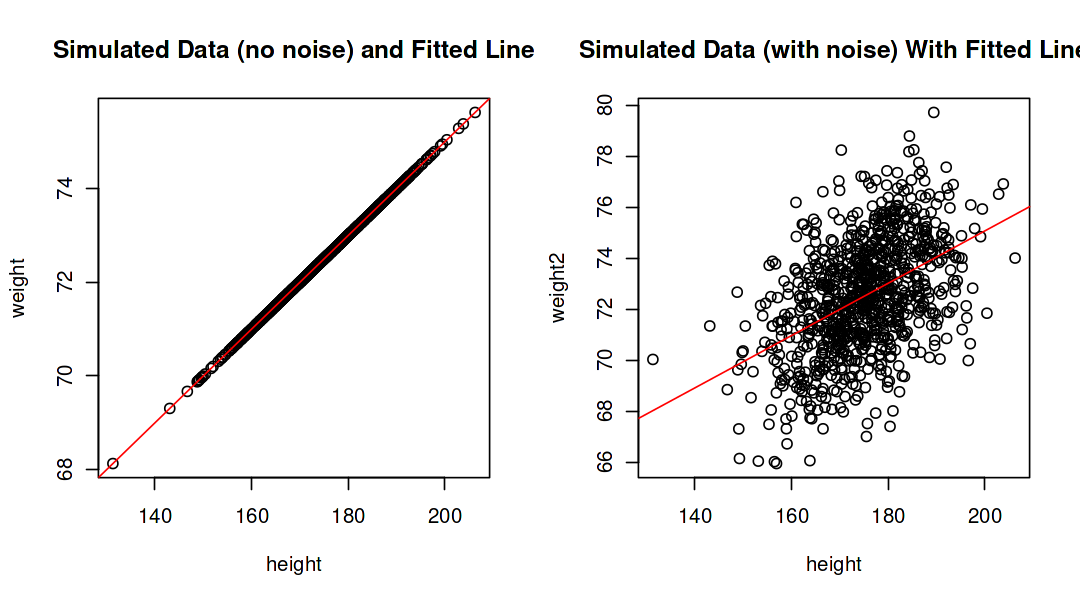
\includegraphics[width=0.95\textwidth]{./figures/reg_figure1.png}
  \caption{Simulated Data Without or With Noise}
\end{figure}


\subsection{3.1 Control Variables}

Now, let's add some control variables to the model. We will add a categorical
variable called \texttt{gender}:

\begin{itemize}
  \tightlist
  \item for female, the distribution of height might be different from male
  \item the relationship between height and weight is different for female and male
\end{itemize}


\begin{lstlisting}
# generate height for female
height_female <- rnorm(450, 170, 5)
female_character <- rep("female", 450)
height_male <- rnorm(450, 175, 10)
male_character <- rep('male', 450)
# put them together as a data.frame and then conver it to the data.table
sim_data <- data.frame(height = c(height_female, height_male), gender = c(female_character, male_character))
sim_data <- as.data.table(sim_data)
head(sim_data)

# add weight 
sim_data %>%
    #[i, j, by]
    .[, weight := ifelse(gender=="female",
                                  50 + 0.09 *height,
                                  55 + 0.1 * height)] -> sim_data2

str(sim_data2)
\end{lstlisting}

Let's review what we have done:

\begin{enumerate}
  \item simulate one variable (height, follows the normal distribution)
  $$height \sim N(175, 10)$$
  \item assume there is a perfect linear relationship between weight and height such as
  $$ weight = 55 + 0.1 * height  $$
  \item add noise into the data because there is no perfect thing in the real life
  $$
weight = 55 + 0.1 * height + \epsilon; \quad \epsilon \sim N(0, 2)
$$
\item bring one more variable into our analysis, let's say gender (female/male)
\item for female, the distribution of height might be different from male
$$
height_f \sim N(170, 5); \quad height_m \sim N(175, 10)
$$
\item the relationship between height and weight is different for female and male
$$
weight_f = 50 + 0.09 * height_f; \quad weight_m = 55 + 0.1 * height_m
$$
\end{enumerate}

You can see that the complexity has already kicks in even for onlhy three variables. Please
run the following code and take a look at the figure.

\begin{lstlisting}
sim_data2 %>%
  ggplot(aes(x=height, y=weight, color=gender)) + 
  geom_point()
\end{lstlisting}

Now, we will fit two regression models, one is simple linear regression model: 


$$
weight = \beta_0 + \beta_1 height + \epsilon; \quad \epsilon \sim N(0, sd)
$$

and the other one is multiple linear regression model (with a control variable):

$$
weight = \beta_0 + \beta_1 height + \beta_2 gender + \epsilon
$$

\begin{table}[!htbp] \centering 
  \caption{Linear Regression Results} 
  \label{} 
\begin{tabular}{@{\extracolsep{5pt}}lcc} 
\\[-1.8ex]\hline 
\hline \\[-1.8ex] 
 & \multicolumn{2}{c}{\textit{Dependent variable:}} \\ 
\cline{2-3} 
\\[-1.8ex] & \multicolumn{2}{c}{weight} \\ 
\\[-1.8ex] & (1) & (2)\\ 
\hline \\[-1.8ex] 
 height & 0.222$^{***}$ & 0.098$^{***}$ \\ 
  & (0.012) & (0.0001) \\ 
  & & \\ 
 gendermale &  & 6.713$^{***}$ \\ 
  &  & (0.002) \\ 
  & & \\ 
 Constant & 30.472$^{***}$ & 48.603$^{***}$ \\ 
  & (2.163) & (0.022) \\ 
  & & \\ 
\hline \\[-1.8ex] 
Observations & 900 & 900 \\ 
R$^{2}$ & 0.261 & 1.000 \\ 
Adjusted R$^{2}$ & 0.260 & 1.000 \\ 
Residual Std. Error & 3.189 (df = 898) & 0.031 (df = 897) \\ 
F Statistic & 317.177$^{***}$ (df = 1; 898) & 6,389,261.000$^{***}$ (df = 2; 897) \\ 
\hline 
\hline \\[-1.8ex] 
\textit{Note:}  & \multicolumn{2}{r}{$^{*}$p$<$0.1; $^{**}$p$<$0.05; $^{***}$p$<$0.01} \\ 
\end{tabular} 
\end{table} 

\begin{figure}[!htbp]
  \centering
  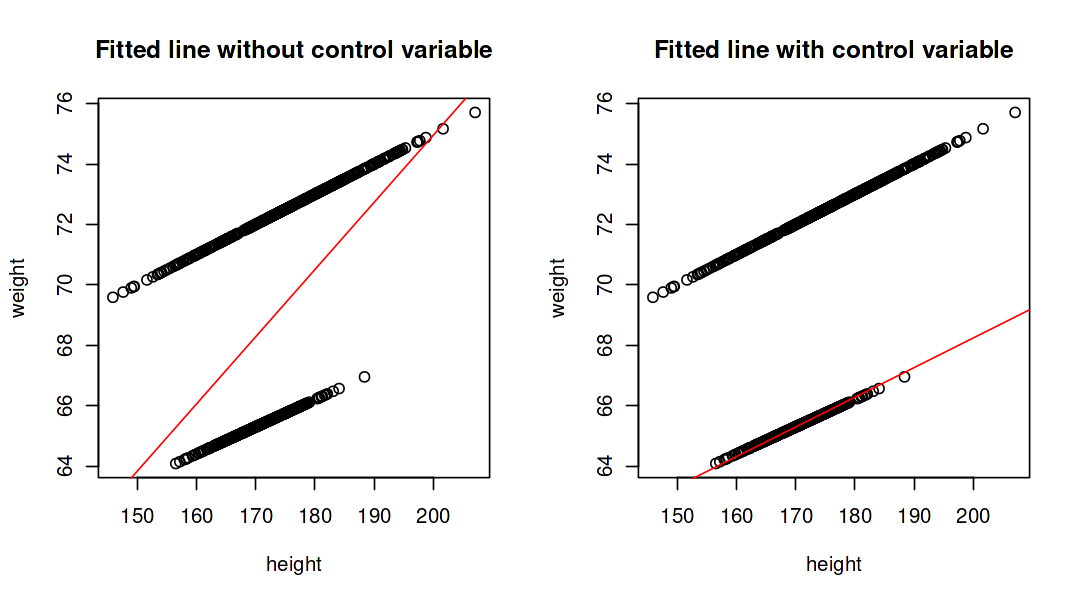
\includegraphics[width=0.95\textwidth]{./figures/reg_figure2.png}
  \caption{Simulated Data and Fitted Regression Line}
\end{figure}

As you can see, the simple linear regression model is not good enough to 
capture the relationship between weight and height. The multiple linear
regression model is better than the simple linear regression model.

\subsection{3.2 Interpretation of Regression Results}

It is very important to know how to interpret the regression analysis results.
 Again, here we are not talking about the causal relationship, 
 but the association between the dependent variable and independent variables. 
 We will use an example to show you.

The dataset we will explore is about the relationship between wage and education. 
Based on our common sense, it is likely that the more education is 
usually \textbf{associated} with higher wage.

\begin{lstlisting}
# install a new package called wooldridge
install.packages("wooldridge")
library(wooldridge)
# load the data
data("wage1")
# convert it to data.table
wage1 <- as.data.table(wage1)
head(wage1)
\end{lstlisting}

As we can see that we have many variables. However,  however we are mainly interested 
in the relationship between wage and education, so we will only focus 
on these two variables and other control variables such as:

\begin{itemize}
  \tightlist
  \item wage: average hourly earnings
  \item educ: years of education
  \item exper: years of experience
  \item female: =1 if female otherwise =0
\end{itemize}

\begin{lstlisting}
# univariate anlaysis
wage1 %>%
    with(hist(wage))
# bivariate analysis
wage1 %>%
     with(plot(educ, wage))
# run regression
wage_reg1 <- lm(wage ~ educ, data=wage1)
stargazer(wage_reg1, type="text")
# bivariate: experience and wage 
wage1 %>%
    with(plot(exper, wage))
# let's run another regression 
wage_reg2 <- lm(wage ~ educ + exper, data=wage1)
stargazer(wage_reg2, type="text")
# let's add non-linear term
wage_reg3 <- lm(wage ~ educ + exper + I(exper^2), data=wage1)
stargazer(wage_reg1, wage_reg2, wage_reg3, type="text")
\end{lstlisting}

\begin{table}[!htbp] \centering 
  \caption{Regression Models for Wage} 
  \label{} 
\begin{tabular}{@{\extracolsep{5pt}}lccc} 
\\[-1.8ex]\hline 
\hline \\[-1.8ex] 
 & \multicolumn{3}{c}{\textit{Dependent variable:}} \\ 
\cline{2-4} 
\\[-1.8ex] & \multicolumn{3}{c}{wage} \\ 
\\[-1.8ex] & (1) & (2) & (3)\\ 
\hline \\[-1.8ex] 
 educ & 0.541$^{***}$ & 0.644$^{***}$ & 0.595$^{***}$ \\ 
  & (0.053) & (0.054) & (0.053) \\ 
  & & & \\ 
 exper &  & 0.070$^{***}$ & 0.268$^{***}$ \\ 
  &  & (0.011) & (0.037) \\ 
  & & & \\ 
 exper$\hat{\mkern6mu}$2 &  &  & $-$0.005$^{***}$ \\ 
  &  &  & (0.001) \\ 
  & & & \\ 
 Constant & $-$0.905 & $-$3.391$^{***}$ & $-$3.965$^{***}$ \\ 
  & (0.685) & (0.767) & (0.752) \\ 
  & & & \\ 
\hline \\[-1.8ex] 
Observations & 526 & 526 & 526 \\ 
R$^{2}$ & 0.165 & 0.225 & 0.269 \\ 
Adjusted R$^{2}$ & 0.163 & 0.222 & 0.265 \\ 
Residual Std. Error & 3.378 (df = 524) & 3.257 (df = 523) & 3.166 (df = 522) \\ 
F Statistic & 103.363$^{***}$ (df = 1; 524) & 75.990$^{***}$ (df = 2; 523) & 64.109$^{***}$ (df = 3; 522) \\ 
\hline 
\hline \\[-1.8ex] 
\textit{Note:}  & \multicolumn{3}{r}{$^{*}$p$<$0.1; $^{**}$p$<$0.05; $^{***}$p$<$0.01} \\ 
\end{tabular} 
\end{table} 


With this model, here is how we will interpret the results: holding other factors
constant, an increase in education of 1 year is associated with an 
increase of 0.595 dollar an hour in wage. The coefficient is significant 
at 1\% level. For experience, we can say that holding other factors constant, 
there is an nonlinear relationship between experience and wage. 
The wage will increase with experience, but it will stop after reaching a certain level.

The coefficients for exper and $exper^2$ are  $0.268$ and  $−0.005$, 
now let's plot the relationship between wage and exper holding 
other factors constant. This means we can have the following equation:


\begin{equation}
wage = 0.268 \times exper - 0.005 \times exper^2 \tag{wage-equation (1)}
\end{equation}

\begin{lstlisting}
# simulate experience from 0 to 40 years
# seq = sequence generated from 0 to 30 with interval 1
exper_seq <- seq(0, 40, 1)
# ^2 means square
wage_sim <- 0.268 * exper_seq - 0.005 * exper_seq^2
# plot the relationship
plot(exper_seq, wage_sim, type="l")
# add vertical line
abline(v=27, col='red')
# we can put them together
wage1 %>%
    with(plot(exper, wage)) +
    lines(exper_seq, wage_sim, type="l", col='red')
# let's simulate other equation
wage_sim2 <- 10 + 0.268 * exper_seq - 0.005 * exper_seq^2

# then we plot it again 
wage1 %>%
    with(plot(exper, wage, main = "Wage and Experience with Equation (2)")) +
    lines(exper_seq, wage_sim2, type="l", col='red') + 
    lines(exper_seq, wage_sim, type="l", col='blue') 
\end{lstlisting}

Why the red curve above does not fit with the dataset exactly? Wage 
is real-lfe data, it is determined:

\begin{itemize}
  \tightlist
  \item educ
  \item experience
  \item industry
  \item networking
  \item etc.
\end{itemize}


Here we only plot the relationship between wage and exper without 
considering other factors. Be aware that wage is the average 
hourly earnings, which is from the real data. wage is determined 
by many factors, such as education and industry. 
Now, image let's assume the wage was determined by the following equaion:


\begin{equation}
wage = 10+  0.268 \times exper - 0.005 \times exper^2 \tag{wage-equation (2)}
\end{equation}

This means that we have nonlinear relationship between
wage and experience. The wage will increase with experience, but it will 
stop after reaching a certain level. Then, no matter what kind of industry you are in,
or degree you have, the relationship between wage and experience will be the 
same and everyone will be added $10$ dollars per hour as a constant.


\begin{figure}[!htbp]
  \centering
  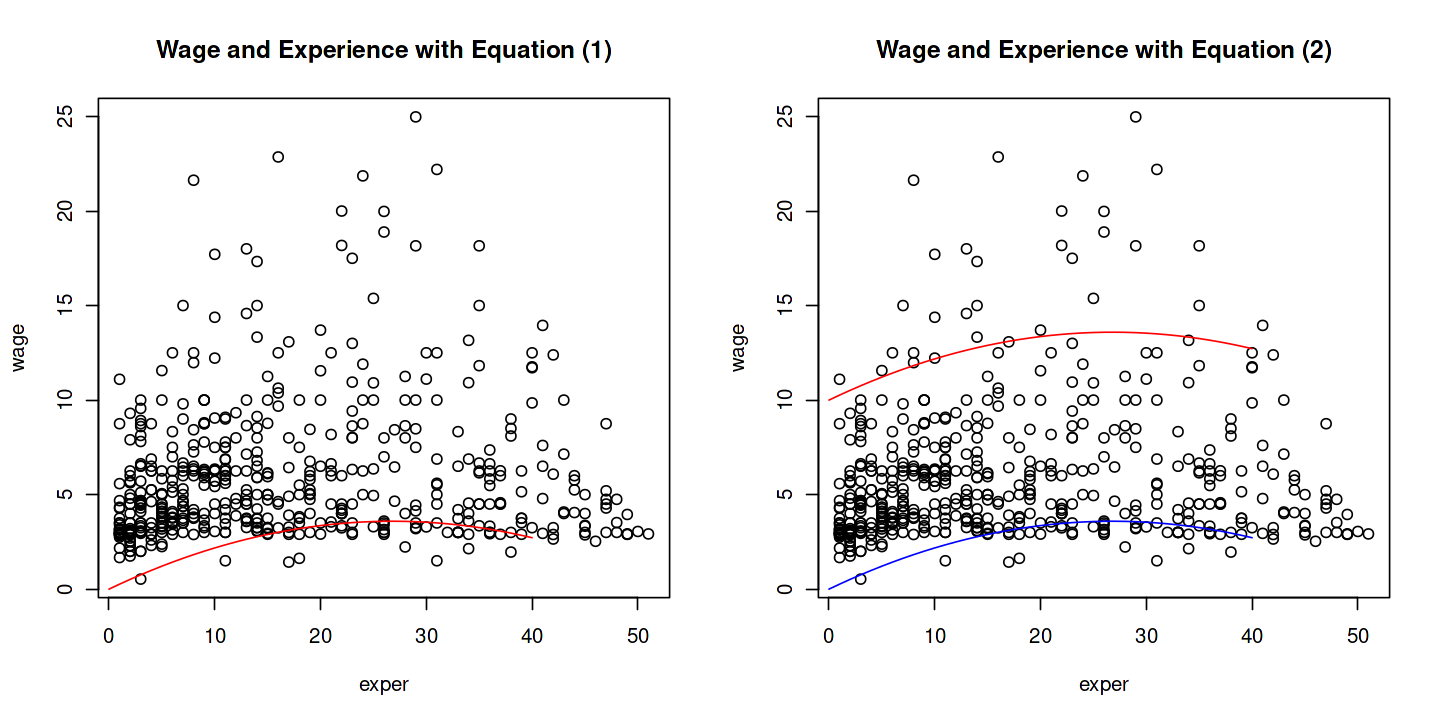
\includegraphics[width=0.95\textwidth]{./figures/reg_figure3.png}
  \caption{Nolinear relationship illustration}
\end{figure}


We have controled the experience, here is the short summary of the regression results. 

The regression results are not causal, but they are useful for us to understand 
the relationship between dependent variable and independent variables.
 Here we can be very confident to say that holding other factors constant, 
 there is a very strong positive association between education and wage. 
 The reason is that the coefficient of education did not change much
when we add more control variables (such as experience). This means whether 
for people who have more experience or not, the education is still positively 
associated with wage.

Now, how about the gender? Does the relationship still hold for different genders? 
Let's run another regression analysis.

\begin{lstlisting}
# add gender in the regression
wage_reg4 <- lm(wage ~ educ + exper + I(exper^2) + female, data=wage1)
stargazer(wage_reg4, type="text")
\end{lstlisting}

\begin{table}[h] \centering 
  \caption{} 
  \label{} 
\begin{tabular}{@{\extracolsep{5pt}}lccc} 
\\[-1.8ex]\hline 
\hline \\[-1.8ex] 
 & \multicolumn{3}{c}{\textit{Dependent variable:}} \\ 
\cline{2-4} 
\\[-1.8ex] & \multicolumn{3}{c}{wage} \\ 
\\[-1.8ex] & (1) & (2) & (3)\\ 
\hline \\[-1.8ex] 
 educ & 0.644$^{***}$ & 0.595$^{***}$ & 0.556$^{***}$ \\ 
  & (0.054) & (0.053) & (0.050) \\ 
  & & & \\ 
 exper & 0.070$^{***}$ & 0.268$^{***}$ & 0.255$^{***}$ \\ 
  & (0.011) & (0.037) & (0.035) \\ 
  & & & \\ 
 I(exper$\hat{\mkern6mu}$2) &  & $-$0.005$^{***}$ & $-$0.004$^{***}$ \\ 
  &  & (0.001) & (0.001) \\ 
  & & & \\ 
 female &  &  & $-$2.114$^{***}$ \\ 
  &  &  & (0.263) \\ 
  & & & \\ 
 Constant & $-$3.391$^{***}$ & $-$3.965$^{***}$ & $-$2.319$^{***}$ \\ 
  & (0.767) & (0.752) & (0.739) \\ 
  & & & \\ 
\hline \\[-1.8ex] 
Observations & 526 & 526 & 526 \\ 
R$^{2}$ & 0.225 & 0.269 & 0.350 \\ 
Adjusted R$^{2}$ & 0.222 & 0.265 & 0.345 \\ 
Residual Std. Error & 3.257 (df = 523) & 3.166 (df = 522) & 2.989 (df = 521) \\ 
F Statistic & 75.990$^{***}$ (df = 2; 523) & 64.109$^{***}$ (df = 3; 522) & 70.170$^{***}$ (df = 4; 521) \\ 
\hline 
\hline \\[-1.8ex] 
\textit{Note:}  & \multicolumn{3}{r}{$^{*}$p$<$0.1; $^{**}$p$<$0.05; $^{***}$p$<$0.01} \\ 
\end{tabular} 
\end{table} 

Here we notice that the coefficient for female is  $-2.114$, 
which means holding other factors constant, women is associated with 
a decrease of 2.114 dollar an hour in wage comparing to men. This 
means even with same education, experience, there is still negative 
association between being female and wage. Therefore, we can say this 
might be due to the gender discrimination in the labor market.

\subsection{3.3 Regression Diagnostics}


Robustness check is a very important concept in regression analysis. 
It is very important to check whether the results are robust to 
different specifications. For instance, we can run the regression analysis 
with different control variables. If the results are robust, then we 
can be more confident about the results.


After running the regression analysis, we need to check whether the results are 
reliable. There are many ways to check the reliability of the results. 
Here we will introduce three ways to check the reliability of the results:

\begin{itemize}
  \tightlist
  \item residual plot: the residual plot is used to check whether the residuals are randomly distributed. If the residuals are randomly distributed, then we can say the results are reliable. Otherwise, we need to check the model specification. For instance, we might need to add more control variables to the model.
  \item VIF: VIF is used to check whether there is multicollinearity in the model. If the VIF is larger than 10, then we need to check whether there is multicollinearity in the model. If there is multicollinearity, then we need to remove some variables from the model.
  \item influential points: influential points are extreme values that deviate from other observations on data , they may indicate a variability in a measurement, experimental errors or a novelty. If there are some influential points, then we need to check whether they are correct. If they are correct, then we need to run the regression analysis again without those influential points.
\end{itemize}


Please run the following code and check the results.

\begin{lstlisting}
install.packages("performance")
install.packages("see")
install.packages("patchwork")
install.packages("wooldridge")
library(performance)
library(wooldridge)

# high influential points
data("infmrt")
str(infmrt)
infmrt <- as.data.table(infmrt)
infmrt %>%
    .[lphysic <= 6.0] %>%
    .[, .(infmort, lpcinc, lphysic, lpopul)] -> infmrt2 

head(infmrt2)
infmrt %>%
    with(plot(lphysic, infmort))
infmrt_reg1 <- lm(infmort ~ lpcinc + lphysic + lpopul, data = infmrt)
stargazer(infmrt_reg1, type="text")
check_model(infmrt_reg1)
infmrt_reg2 <- lm(infmort ~ lpcinc + lphysic + lpopul, data = infmrt2)
stargazer(infmrt_reg2, type="text")
check_model(infmrt_reg2)

# multicollinearity
elem_data <- fread("https://shorturl.at/awLNT")
head(elem_data)
str(elem_data)
elem_reg1 <- lm(api00 ~ acs_k3 + avg_ed +  grad_sch + col_grad + some_col, data = elem_data)
stargazer(elem_reg1, type='text')
options(repr.plot.width = 11, repr.plot.height = 8)
check_model(elem_reg1)
\end{lstlisting}





\section{4 Multiple Linear Regression}

To summarize what we have learned, we have the following regression models:

\begin{equation}
  y = \beta_0 + \beta_1 x_1 + \beta_2 x_2 + \cdots + \beta_k x_k + \epsilon
\end{equation}

where

\begin{itemize}
  \tightlist
  \item $y$ is the dependent variable
  \item $x_1, x_2, \cdots, x_k$ are independent variables
  \item $\beta_0, \beta_1, \cdots, \beta_k$ are coefficients
  \item $\epsilon$ is the error term
\end{itemize}

We assume assume the following assumptions. 


\begin{table*}[!htb]
  \centering
  \begin{tabular}{ll}
    \hline 
    \hline 
    Assumptions & Diagnostic check \\ 
    \hline 
    A1: linear relationships between $y$ and each $x$ & check via plots\\
    A2: Independence of observations & check via plots  \\
    A3: $E(\epsilon | x) = 0$ & check via plots \\ 
    A4: $Var(\epsilon | x) = \sigma^2$ & check via plots  \\
    A5: Normality of the error $\epsilon \sim N(0, \sigma^2)$ & check via plots  \\
    A6: No correlation between $x$ and $\epsilon$: $cor(x, \epsilon)=0$ & serial correlation test \\ 
    \hline 
  \end{tabular}
  \caption{A summary of model assumptions and regression diagnostic}
\end{table*}


\begin{figure}[!htbp]
  \centering
  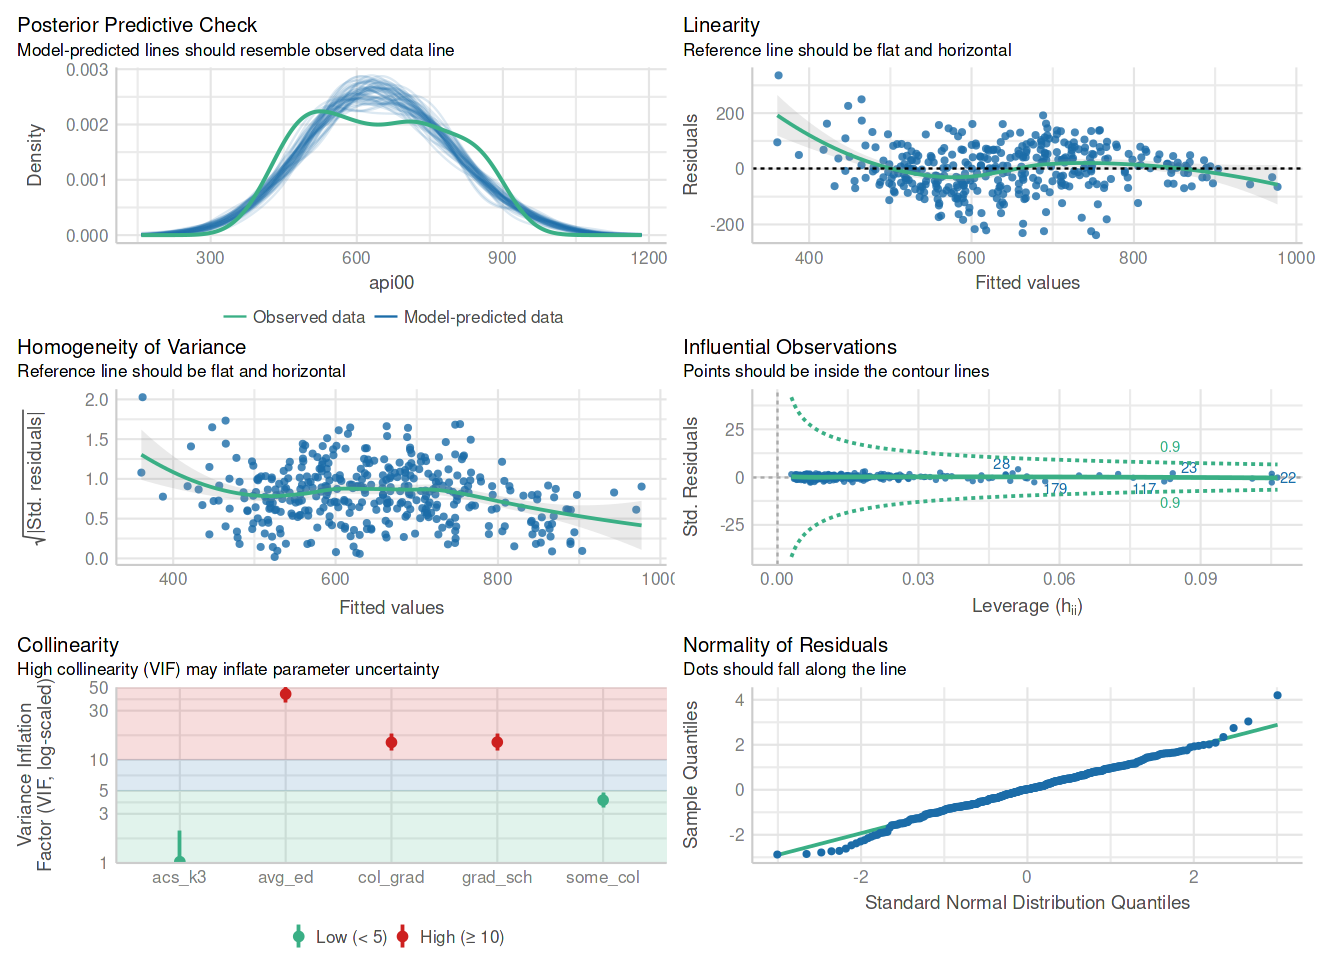
\includegraphics[width=0.95\textwidth]{./figures/reg_figure4.png}
  \caption{Regression Diagnostics Plots}
\end{figure}


\section{5 Logistic Regression}

You will not tested on logistic regression in the exam. However, it is very important
to know when the dependent variable is not continuous. For instance, if the dependent
variable is binary, then we can use logistic regression.

You can follow this link \url{https://daviddalpiaz.github.io/r4sl/logistic-regression.html}
to learn more about logistic regression.


\section{6 Please Read the Following Materials}





\end{document}